\chapter{JavaScript}

JavaScript is een scripttaal die werd ontwikkeld om op webpagina's interactie mogelijk te maken met gebruikers.
Voor dit vak is JavaScript alleen maar een middel om het doel (Leren Programmeren) te bereiken.
De bedoeling is dat jullie leren algoritmisch na te denken, dat jullie leren werken met verschillende
controle-structuren, met verschillende data-types,... JavaScript is \'e\'en van de vele mogelijke middelen
om het uiteindelijke doel te bereiken. Het heeft als grote voordeel dat er weinig tot geen hulpmiddelen nodig
zijn om aan de slag te gaan: een eenvoudig HTML-sjabloontje volstaat. Als je in het HTML-sjabloon je code typt,
met in acht neming van enkele taal-specifieke regels, kan je je code eenvoudigweg uitvoeren door je HTML-file
te openen in een browser.

\htmlcodefigure[basicstyle=\small]{JavaScript/skeleton.html}{Een eenvoudige HTML-pagina met een script.}{lst:html}

\section{JavaScript versus Java}

JavaScript is niet hetzelfde als Java. Hier vind je een overzicht van enkele verschillen:

\begin{enumerate}
\item Java is een programmeertaal waarvan je de programmacode moet compileren, terwijl Javascript een scripttaal is waarvan de programmacode door de browser op de computer van de eindgebruiker wordt ge\"interpreteerd.
\item De broncode in JavaScript is normaal gesproken volledig in HTML-documenten ingebed terwijl bij een Java-applet alleen maar een tag om de applet uit te voeren in de HTML-code wordt opgenomen (een java-applet is gecompileerde broncode).
\item In Java moet je variabelen declareren, net als in hogere programmeertalen als C of C++. Bovendien moet je het type variabele zelf toewijzen ( tekenreeks, getal ). In JavaScript moet je variabelen echter niet declareren. Dit wil zeggen dat een variabele automatisch door JavaScript wordt gedefini\"eerd wanneer je dat niet zelf doet. Het type variabele kan je tijdens de uitvoering van het programma veranderen.
% \item JavaScript gebruikt dynamic-binding terwijl Java static-binding toepast. Static-binding betekent dat de Java-compiler reeds tijdens het compileren, dat wil zeggen tijdens de omzetting in machinetaal, de verwijzingen naar objecten controleert. Bij JavaScript zijn deze verwijzingen dynamisch en kunnen ze zelfs nog worden veranderd tijdens de uitvoering van het programma.
\end{enumerate}

Java en JavaScript komen natuurlijk op een aantal punten wel overeen. Zo zijn ze bijvoorbeeld syntactisch heel gelijkaardig en zijn ze beide hoofdlettergevoelig.

\section{Variabelen}

Een programma dat iets moet berekenen, gaat plaats nodig hebben in het werkgeheugen van de computer om (tussen)resultaten op te slaan. Deze plaatsen in het geheugen noemen we `variabelen'. Afhankelijk van welke data je in een stukje geheugen wil opslaan, hebben de variabelen een bepaald type. Zo zijn er variabelen waar bijvoorbeeld tekst wordt in opgeslaan, of een datum, een getal, een boolse waarde (\inlinecode{true} of \inlinecode{false}), ...

In een sterk-getypeerde taal zoals Java moet je bij het aanmaken van een variabele expliciet zeggen welk type data er in die variabele opgeslagen mag worden. Zo kan je een variabele van type `int' aanmaken, waar enkel gehele getallen in opgeslagen kunnen worden. JavaScript werkt echter anders: variabelen kunnen elk type van data bevatten. Op \'e\'en moment kan een variabele natuurlijk maar \'e\'en type van data bevatten, maar je kan later in dezelfde variabele een stukje data opslaan van een ander type. Wanneer je in JavaScript een variabele aanmaakt, moet je dus niet aangeven van welk type die variabele moet zijn.

\examplecode{JavaScript/varexample.js}

Het stukje code hierboven maakt een aantal variabelen aan. De vetgedrukte woorden zijn sleutelwoorden van JavaScript. Dit zijn woorden met een speciale betekenis. In dit geval zegt het sleutelwoord var dat er een variabele moet aangemaakt worden met een naam die volgt (`getal', `tekst', ...). Bij het aanmaken van een variabele kan er onmiddellijk ook een initi\"ele waarde aan toegekend worden. De waarde die achter het gelijkheidsteken staat wordt gezet in het geheugenplaatsje van de variabele. Je moet hier het gelijkheidsteken zien als een toekenning van wat er aan de rechterkant van het gelijkheidsteken staat aan wat er aan de linkerkant van het gelijkheidsteken staat. Verder zien we nog dat een lijn in JavaScript doorgaans met een puntkomma wordt afgesloten. JavaScript dwingt dit niet af, maar het wordt heel sterk aangeraden om te doen. Java dwingt dit wel af, dus als je altijd puntkommas gebruikt aan het einde van je lijnen code, dan zal je in Java hiertegen geen fouten maken.

De eerste lijn maakt een variabele met de naam `getal' aan en steekt hier de waarde 10 in. De tweede lijn maakt de variabele `tekst' aan en steekt hier het stukje tekst ``Hallo'' in. Merk op dat deze initi\"ele tekst tussen dubbele aanhalingstekens staat. Telkens als we in JavaScript tekstuele data gebruiken zullen we die tussen dubbele haakjes zetten. Een variabele met tekst in, wordt ook wel een string genoemd. De derde lijn maakt een variabele `isDitLeuk' aan, en kent er de boolse waarde `true' aan toe. een boolse waarde kan enkel `true' of `false' zijn. Lijn vier maakt een variabele `nogNiets' aan en initialiseert deze nog niet. Hij zal dus initieel leeg blijven.

De vijfde lijn uiteindelijk zal de waarde van de variabele die we eerder aangemaakt hadden aanpassen en op `3.14' zetten. Merk op dat het kommagetal geschreven wordt met de Amerikaanse schrijfwijze (d.w.z. er wordt een punt gebruikt). De variabele `getal' is aangemaakt op lijn 1 van het programma. We moeten op lijn 5 dus niet opnieuw het sleutelwoord var gebruiken, aangezien  de variabele reeds bestaat.

Ons programma moet natuurlijk ook kunnen werken met deze variabelen. Afhankelijk van het datatype kan je bepaalde operaties op variabelen uitvoeren. (Zo kan je bijvoorbeeld twee getallen delen, maar twee stukjes tekst kan je niet delen.)

Op getallen kunnen we de standaard wiskundige operaties uitvoeren. Zo kunnen we twee getallen optellen, aftrekken, vermenigvuldigen of delen. Enkele voorbeelden:

\examplecode{JavaScript/mathexample.js}

De lijnen die beginnen met // zijn commentaarregels. Alles tekst die op dezelfde lijn achter de // staat zal genegeerd worden tijdens de uitvoering van het programma.

Merk op dat we veelvuldig gebruik maken van de toekenningsoperator (het gelijkheidsteken) omdat anders onze berekende waardes worden weggegooid. Bijvoorbeeld, op de derde lijn zal alles wat langs de rechterkant van het gelijkheidsteken staat gestoken worden in de variabele die langs de linkerkant van het gelijkheidsteken staat. Langs de rechterkant staat ``getal + 5''. Tijdens de uitvoering van het programma zal gekeken worden welke waarde op dat moment in de variabele getal staat, en bij deze waarde zal 5 opgeteld worden. Dit tussenresultaat wordt dan gestoken in de variabele die voor het gelijkheidsteken staat. Het uiteindelijke resultaat van deze lijn code is dat de waarde van getal met vijf verhoogd wordt.

Een andere wiskundige operatie die we vaak gaan gebruiken in de oefeningen is de modulo-operator. Hiermee kunnen we de `rest bij deling' berekenen. In JavaScript wordt de modulo-operator genoteerd met een procentteken. Indien we de rest willen berekenen van een deling van het getal 10 door 4, en dit resultaat willen opslaan in een variabele, kunnen we dat als volgt noteren in JavaScript: \inlinecode{var rest = 10 \% 4}.
De waarde van de variabele \inlinecode{rest} zal 2 zijn, aangezien de rest
van de deling van 10 door 4 inderdaad 2 is.

Indien je een variabele wil verhogen, verlagen, delen of vermenigvuldigen met een ander getal (en het resultaat dan terug in de originele variabele zetten), dan kan je de code iets compacter schrijven. Zo zijn de bovenstaande operaties ook te schrijven als volgt:

\examplecode{JavaScript/mathassign.js}

In deze code zal de variabele `getal' dus verhoogd, vermenigvuldigd, gedeeld en verlaagd worden, en zal het berekende resultaat telkens terug in `getal' opgeslagen worden. Indien je een variabele met 1 wil verhogen of verlagen, kan het zelfs nog korter:

\examplecode{JavaScript/incdec.js}

\section{Ingebouwde methodes}

JavaScript bevat een aantal ingebouwde methodes die het leven van de programmeur een stuk makkelijker kunnen maken. Deze methodes kunnen opgeroepen worden om een bepaalde taak uit te voeren. Hieronder bespreken we een aantal van deze methodes die we in de oefeningen regelmatig zullen gebruiken.

\subsection{Invoer}

Onze programma's gaan met de gebruiker moeten interageren door bijvoorbeeld invoer te vragen of een resultaat te tonen. We kunnen in JavaScript invoer vragen door gebruik te maken van de prompt-methode. Deze methode toont een invoerscherm aan de gebruiker, waar die dan iets kan intypen.

\examplecode{JavaScript/prompt.js}

Zo geeft de bovenstaande lijn code het resultaat in Figuur~\ref{fig:prompt}

\begin{figure}
\centering
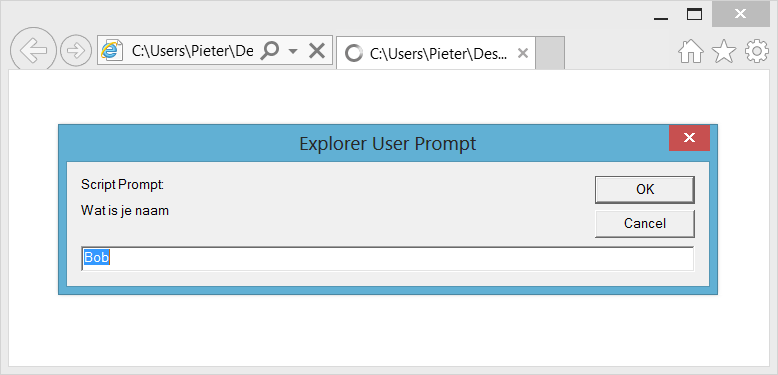
\includegraphics[scale=0.8]{JavaScript/prompt.png}
\caption{Een JavaScript prompt}\label{fig:prompt}
\end{figure}

Je roept de prompt-methode op door zijn naam te schrijven. Aan de methode kunnen twee parameters meegegeven staan (die tussen haakjes achter de methodeoproep staan, gescheiden door een komma). De eerste parameter is een verplichte parameter waar je de tekst doorgeeft die getoond wordt aan de gebruiker. De tweede parameter is optioneel en bevat de standaardwaarde.

Van zodra de gebruiker op OK klikt, zal zijn invoer teruggegeven worden als het resultaat van de prompt-oproep. In bovenstaande code wordt dit resultaat dan gestoken in de variabele `invoer'.

Je programma moet ook uitvoer kunnen tonen aan de gebruiker. Hier kan je de alert-methode voor gebruiken, die \'e\'en parameter verwacht: het bericht dat je aan de gebruiker wil tonen.

\examplecode{JavaScript/alert.js}

De bovenstaande lijn code geeft het resultaat in Figuur~\ref{fig:alert}.

\begin{figure}
\centering
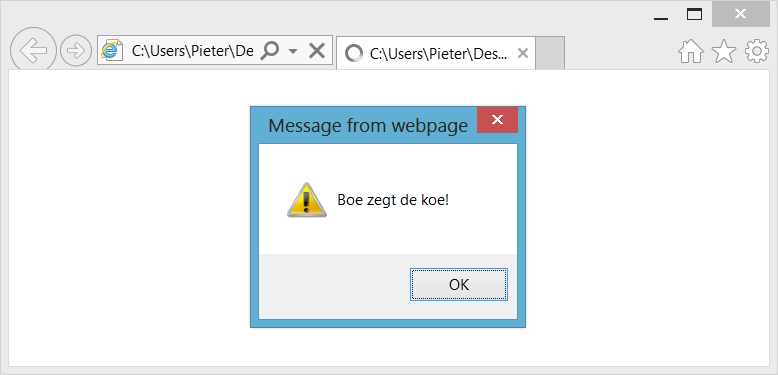
\includegraphics[scale=0.8]{JavaScript/alert.png}
\caption{Een JavaScript alert}\label{fig:alert}
\end{figure}

\subsection{Tekst}

Variabelen met tekst in willen we ook kunnen bewerken. JavaScript biedt ons een aantal methods aan die we hier voor kunnen gebruiken. Zo heeft een variabele met tekst een eigenschap die de lengte van die tekst teruggeeft.

\examplecode{JavaScript/string.js}

In bovenstaande code zal de variabele l de waarde 6 krijgen (omdat de naam uit zes karakters bestaat). Deze length-eigenschap bestaat niet voor variabelen met getallen of boolse waardes.

We kunnen ook een bepaald karakter opvragen uit een tekst door gebruik te maken van de charAt-methode. We geven aan deze methode de locatie mee van welke letter we uit de tekst willen halen. De locatie begint wel vanaf 0 te tellen; het eerste karakter in de tekst staat op plaats 0, het tweede karakter op plaats 1, enz. De indexOf-methode geeft ons de beginlocatie terug van een bepaald stuk (deel)tekst in de hoofdtekst, of de waarde -1 indien de deeltekst niet gevonden is. lastIndexOf doet hetzelfde, maar zoekt in de hoofdtekst van achter naar voor. De substr-methode kan gebruikt worden om uit een stuk tekst een deel te kopieren. Het verwacht twee parameters: de beginpositie van waar gekopieerd moet worden (ook weer te beginnen vanaf 0), en het aantal karakters dat gekopieerd moet worden. Twee stukken tekst kunnen aan elkaar geplakt worden door gebruik te maken van het plusteken.

\examplecode{JavaScript/stringops.js}

De waarde van beginLetter zal na het uitvoeren van deze code op ``B'' staan. locatieIE zal de waarde 3 bevatten. laatsteVier zal de waarde ``bien'' bevatten. aaneenGeplakt zal ``HalloWereld'' zijn.

\subsection{Getallen}
We weten dat we invoer kunnen vragen aan de gebruiker door middel van de prompt-methode. Deze methode zal altijd een variabele van type String teruggeven. Als we dus een getal willen vragen aan de gebruiker, kunnen we hier ook de prompt-methode voor gebruiken, maar krijgen we het getal dat de gebruiker ingegeven heeft in tekstvorm terug. Als we met deze invoer willen rekenen, dan moeten we het eerst converteren naar echt getal.

Gelukkig biedt JavaScript twee methodes aan die we kunnen gebruiken om een tekst met een getal in te converteren naar een getal waar we mee kunnen rekenen. parseInt converteert een tekst naar een geheel getal, terwijl parseFloat een tekst naar een kommagetal omzet.

\examplecode{JavaScript/parse.js}

We kunnen parseInt eventueel op dezelfde lijn combineren met een oproep van prompt. Als we bijvoorbeeld een geheel getal aan de gebruiker willen vragen en opslaan in de variabele getal, dan kunnen we dat schrijven als volgt:

\examplecode{JavaScript/getint.js}

JavaScript gaat de bovenstaande code als volgt interpreteren: maak een variabele `getal' aan, en steek daar het resultaat in van alles wat aan de rechterkant van het gelijkheidsteken staat. Dit is een oproep naar parseInt, waar je als parameter het resultaat van een oproep naar prompt aan meegeeft.

Kommagetallen kunnen afgerond worden naar boven, naar beneden, of naar het dichtstbijzijnde gehele getal. Voor deze drie operaties kan je gebruik maken van de Math.ceil, Math.floor en Math.round methodes. Elk van deze methodes verwacht \'e\'en parameter (een getal), en geeft het resultaat terug.

Soms hebben we ook random getallen nodig, waarvoor de Math.random methode gebruikt kan worden. Deze methode verwacht geen parameters, en geeft telkens een random kommagetal terug tussen 0 en 1 (exclusief 1). Indien je een random getal tussen 0 en 100 (exclusief) wil hebben, kan je het resultaat van Math.random gewoon met 100 vermenigvuldigen.

\section{JavaScript leren}

Deze cursus gebruikt JavaScript om studenten te leren programmeren. Het accent van deze cursus ligt dus op het aanleren van gestructureerd een probleem te analyseren en een implementatie hiervan uit te werken. Het accent ligt dus niet op JavaScript. In het vervolg van deze tekst worden een aantal concepten uitgelegd aan de hand van JavaScript en wordt er ook genoeg informatie gegeven om aan de slag te kunnen met JavaScript als programmeertaal. De informatie die hier beschreven is zal echter eerder beperkt zijn, en een aantal JavaScript-specifieke details worden niet vermeld. Het is dus jullie verantwoordelijkheid om naast deze cursus ook extra informatie op te zoeken over JavaScript en oefeningen te maken die niet in de oefeningenbundel van dit vak beschreven zijn. Gelukkig is er een overvloed aan websites beschikbaar waar je terecht kan voor deze extra informatie.

Aangezien JavaScript veelal gebruikt wordt om webpagina's op te smukken, zullen veel van deze informatiebronnen ook de nadruk leggen op de interactie van JavaScript en webpagina's. Alhoewel jullie natuurlijk vrij zijn (en zelfs aangemoedigd worden!) om hier mee te experimenteren, is het in principe niet de bedoeling van deze cursus.

Enkele webagina's die jullie op weg kunnen helpen zijn:
\begin{itemize}
\item Leren programmeren in JavaScript (tutorials): \url{http://www.codecademy.com}
\item Leren programmeren in JavaScript (vooral modules 1 tot 20 zijn belangrijk): \url{http://thenewboston.org/list.php?cat=10}
\item Een website met een aantal voorbeeldproblemen (de focus ligt niet op JavaScript, maar je kan die problemen natuurlijk wel uitgewerken in JavaScript): \url{http://codingbat.com/}
\item JavaScript tutorials, en een referentie met alle functies die JavaScript standaard aanbiedt aan een programmeur: \url{http://www.w3schools.com/jsref/}
\end{itemize}

%%% Local Variables: 
%%% mode: latex
%%% TeX-master: "../main"
%%% End: 
